\documentclass[7pt,landscape,a4paper]{scrartcl}   	

%Define which packages are used
\usepackage[landscape]{geometry} 		%Paper formatting              		   		
\usepackage{graphicx}	
\usepackage{multicol}				%Use for multiple collumns
\usepackage[ngerman]{babel}
\usepackage[utf8]{inputenc}
\usepackage{mathptmx}
\usepackage{listings}				%Used to display code


%SetPaper
\geometry{top=0.1cm,left=0.1cm,right=0.1cm,bottom=0.1cm} 
\setlength{\columnseprule}{1pt}
%Path relative to the .tex file containing the \includegraphics command
\graphicspath{ {./src/} }

%KOMAoptions
\KOMAoptions{headings=normal}

% -------------------------------------------------------------------------
\begin{document}
% Collumns
\begin{multicols*}{4}

% Title
\section{BSYS1 - Marco Agostini}
\vspace{-1.0em}
%Grundlagen
\subsection{Computermodell}
\vspace{-1.0em}
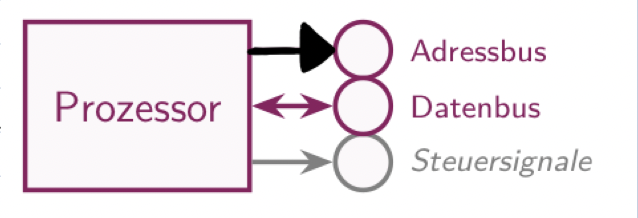
\includegraphics[width=0.5\linewidth]{computermodell}
\begin{minipage}[b]{0,5\linewidth}
\textbf{Computermodell}\\
AB: Adresse\\
DB: Daten\\
SS: Instruktion
\end{minipage}
\includegraphics[width=0.45\linewidth]{Instruktioncodierung}
\begin{minipage}[b]{0,5\linewidth}
Jede Instruktion hat eine eigenen Codierung bestehend aus dem Opcode und den Daten. (Achtung Little Endian!)
\end{minipage}
%Assembler und Daten
\subsection{Assembler}
\vspace{-0.75em}

Der Assembler ist ein Compiler, der textuelle Befehle in Maschienencode übersetzt. (Assembler/Assembly language)
\textbf{Byteweise Adressierung} Intel-Prozessoren addressieren einzelne Bytes. NASM übersetzt jede Anweisung direkt in Binärzahlen und schreibt die Bytesequenz in die Datei.\\
\textbf{Endianes/Byte order}\\
Folgende Daten können spezifiziert werden.\\
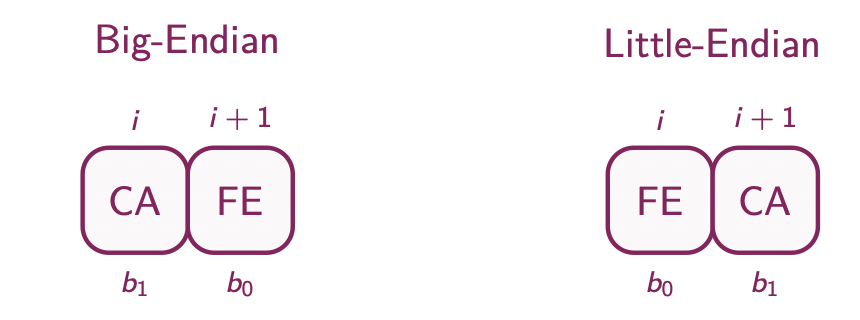
\includegraphics[width=0.45\linewidth]{endian}
\begin{minipage}[b]{0,5\linewidth}
i: Adressen der Bytes\\
b$_{1}$ b$_{2}$: Stellenwerte\\
Word 2Byte, Doubleword 4Byte\\ Quadword 8Byte, D. Quadword 16Byte
\end{minipage}
\textbf{Offset in Byte Sequenzen:} Jedes Byte in der Bytesequenz erhält einen Offset (Adresse/Index). 
\textbf{Labels:} Intern assoziiert der Assembler das Label mit dem Offset des nachfolgenden Befehls. (Wird nicht in Bytecode übersetzt)
\textbf{Flat-Form Binaries (Plain,Pure,Raw)} Bytesequenz analog zum Quelltext.
\textbf{Object-Files} Enthalten neben der Bytesequenz auch noch weiter Informationen: Symboltabelle. Die Symboltabelle assoziiert die Labels mit dem Offset.\\
\textbf{Logische Operationen Assembler}\\
\begin{minipage}[b]{0,3\linewidth}
\begin{verbatim}
not rax
and rax, rbx
or rax, rbx
xor rax, rbx
\end{verbatim}
\end{minipage}\\
%Flags
\textbf{Flags}
Eigenständige Bits, die eine Bedeutung haben. Liegen im gemeinsamen Register RFLAGS, das nicht direkt verwendet werden kann.\\
\begin{minipage}[b]{0,3\linewidth}
CF = Carry Flags\\
OF = Overflow Flag\\
PF = Parity Flag\\
SF = Sign Flag\\
ZF = Zero Flag\\
\end{minipage}
\begin{minipage}[b]{0,7\linewidth}
Überlauf unsigned Arithmetik\\
Überlauf signed Arithmetik\\
Niederwertigstes Byte, gerade Zahl gesetzter Bits\\
Entspricht dem höchstwertigsten Bit\\
Wird gesetzt, wenn das Resultat 0 ist\\
\end{minipage}
%Condition Codes
\textbf{Condition Codes} Definieren eine Bedingung für einen Befehle. Der Befehl wird ausgeführt, wenn der Condition Code TRUE ist.\\
\begin{minipage}[b]{0,5\linewidth}
\begin{verbatim}
mov rax, [p]
cmovnz rax, [q]	
\end{verbatim}
\end{minipage}
\begin{minipage}[b]{0,5\linewidth}
\begin{verbatim}
Sets ZF = 1 if [p] == 0
Sets rax =[q] if [p] != 0 
\end{verbatim}
\end{minipage}
\textit{Compare} Das gleiche wie sub, setzt aber nur die flags.
\textit{Test} Ist ein and ohne Operation und wird verwendet die Register auf 0 zu setzen.\\
\begin{minipage}[b]{0,5\linewidth}
\begin{verbatim}
mov rax, [uy]
mov rbx, [ux]
cmp rax, rbx
cmove rax, 5
\end{verbatim}
\end{minipage}
\begin{minipage}[b]{0,5\linewidth}
\begin{verbatim}
test rax, rbx
cmovz rax, rbx
\end{verbatim}
\end{minipage}\\
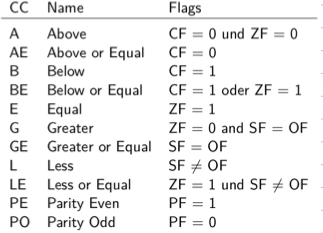
\includegraphics[width=0.5\linewidth]{conditioncodes}
\begin{minipage}[b]{0,5\linewidth}
Signed: L / G\\
Unsigned: B / A
\end{minipage}

%Conditional Jumps
\textbf{Conditional Jumps}
Benötigen einen Condition Code und springen nur wenn dieser erfüllt ist. Vergleich C und Assembly.\\
\begin{minipage}[b]{0,5\linewidth}
\begin{verbatim}
if(ux < 3 ) {
 /* if-body */
 } else {
 /* else-body */ 
 }
\end{verbatim}
\end{minipage}
\begin{minipage}[b]{0,5\linewidth}
\begin{verbatim}
mov eax, [ux]
cmp max, 2
ja else_body
jmp after_if
else_body:
	:else-body
after_if:
\end{verbatim}
\end{minipage}

%Linker
\subsection{Linker} 
\vspace{-0.75em}
Programme werden aus mehreren Assemblerdateien erstellt. Diese Dateien müssen zu einem Executable gelinkt werden. Diese Dateien erhalte eine gemeinsame Symboltabelle.\\
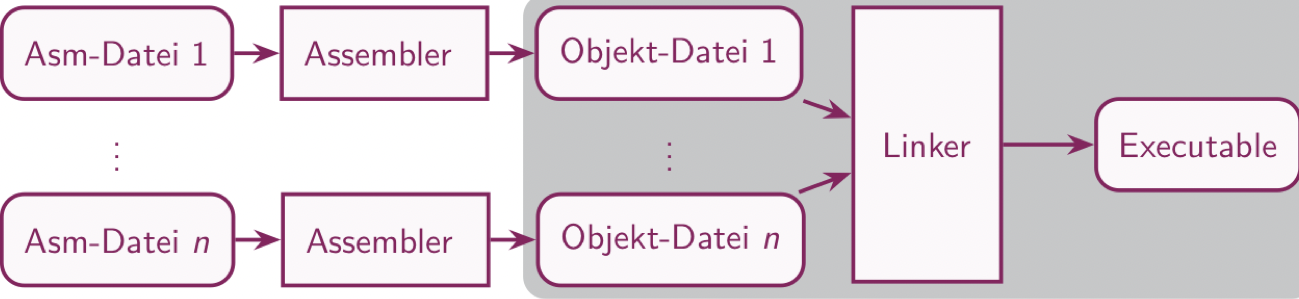
\includegraphics[width=\linewidth]{linker}

%Intel 64 Architektur
\subsection{Intel 64 Architektur}
\vspace{-0.75em}
Ursprünglich hatten die Intel-Prozessoren 16-Bit Register. Auf Intel-64 werden 64 Bit-Register verwendet.\\
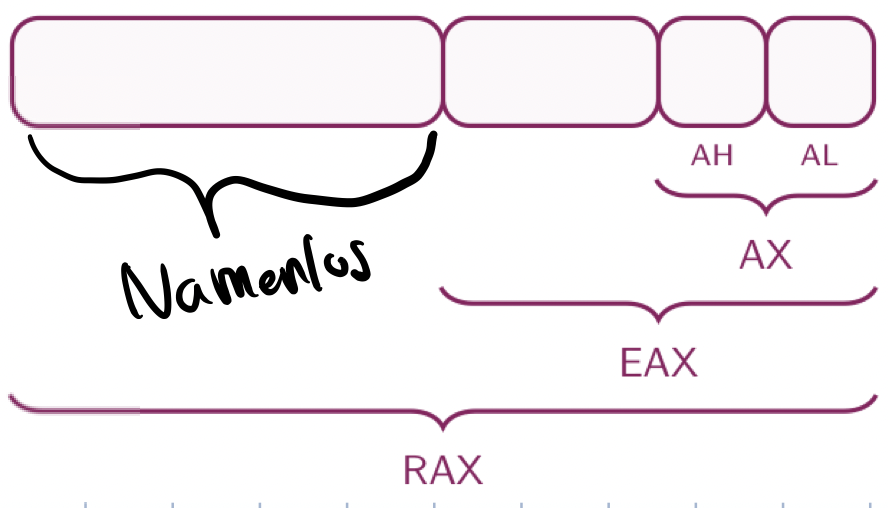
\includegraphics[width=0.5\linewidth]{register}
\begin{minipage}[b]{0,5\linewidth}
RAX: Accumulator\\
RCX: Counter\\
RDX: Pointer für I/O\\
RBX: Basepointer\\
RSI,RDI: Quell und Zielindizes- für Stringopeationen\\
RSP, Stackpointer, Adresse Stack\\
RSB Basepointer, Addresse in Stack\\
R8-R15: Zusätzliche Register
\end{minipage}
\textbf{Länge der Instruktionen:} 1 - 15 Byte
\textbf{Grösse Operanden} Können 8,16,32,64 Bit betragen, müssen aber gleich gross sein (In der gleichen Registergrösse).\\
\textbf{Grundegende Operationen in Assembler}\\
\begin{minipage}[b]{0,35\linewidth}
\begin{verbatim}
mov rax, rbx
mov rax, 0x8000
mov rax, [0x8000]
\end{verbatim}
\end{minipage}
\begin{minipage}[b]{0,65\linewidth}
	Setze Inhalt von rax gleich rbx\\
	Setze rax gleich 8000$_{h}$\\
	Setze rax gleich Speicher 8000$_{h}$ - 8007$_{h}$ 
\end{minipage}
\textbf{Adresierungsmodi}\\
\begin{minipage}[b]{0,35\linewidth}
\begin{verbatim}
mov rax, [0x8000]
mov rbx, 0x8000
mov rax, [rbx]
mov Rex, 0x1000
mov rax, [rcx * 8]
\end{verbatim}
\end{minipage}
\begin{minipage}[b]{0,5\linewidth}
\textbf{Displacement} Adresse \\
\textbf{Base} \\
Adresse steht in einem Register \\
\textbf{Scaled Index} \\Skalierte Adresse
\end{minipage}

%Section C-Toolchain
\vspace{-0.75em}
\subsection{C-Toolchain}
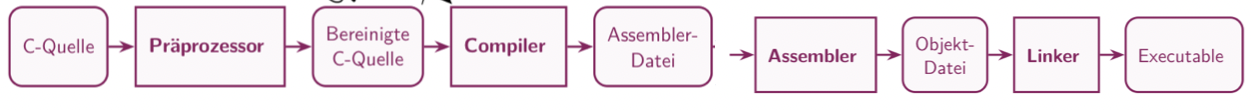
\includegraphics[width=\linewidth]{ctoolchain}
\textbf{C-Sprachebenen}
\textit{Präprozessor:} Definiert Direktiven, die später als Tokenersetzung durchgeführt werden.
\textit{Basiskonstrukte:} Grundgerüst des Programmes: Variablen, Schliefen, Verzweigungen \textit{Standardbibliotheken:} Stellen Funktionen und Typen bereit, die die Basis-Funktionalität enthalten.\\
\textbf{Präprozessor}\\
1. Entfernt Kommentare und wandelt forgesetzte Zeilen in eine Zeile.\\
2. Teilt den gesamten Code in Tokens ein (Tokenization). Der Präpozessor versucht immer die gröstmögliche Tokens zu erstellen.\\
3. Führt Präprozessor-Direktiven aus, ersetzt Makros durch ihre Expansion
\\
%Tokenklassen
\textbf{Token-Klassen}
Bezeichner (Identifier), Präpozessor-Zahlen,String ("Hello") und Char-Literale ('x'), Operatoren und Satzzeichen (punctuators), Sonstige. (Nachfolgend Operatoren und Satzzeichen)\\
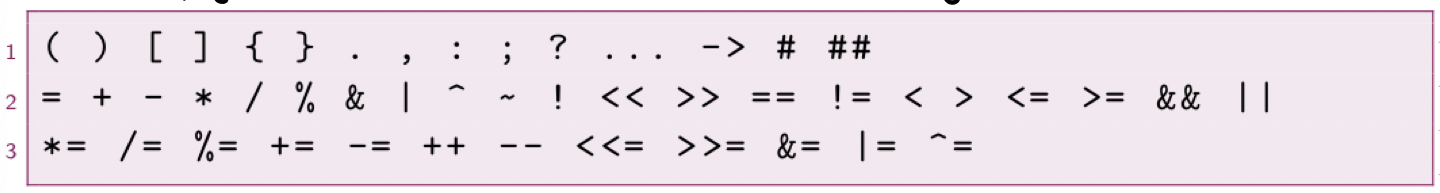
\includegraphics[width=\linewidth]{operatorenundsatzzeichen}\\
\textit{Bezeichner (Identifier)} sind das Gegenstück zu den Labels in Assembler. Bezeichner können deklariert und definiert werden.\\
\textbf{Präprozessor-Direktiven}
Ist das Token auf einer Zeile \#, wird das nächste Token als Direktive interpretiert. Beide Token werden entfernt und die entsprechende Direktive ausgeführt. (\#include, \#define, \#if, \#else, \#endif)\\
\textit{\#Include} Präpozessor öffnet die Datei anhand des nächsten Tokens und führt Durchläufe 1 - 3 für hile.h durch. (\flq file.h\frq  Suche in Systemverzeichnis, \grqq file.h\grqq sucht im aktuellen Verzeichnis + Systemverzeichnis)\\
\textbf{Objektartige Makros} (\#define XYZ 123) Der Präprozessor ersetzt im Programmcode nach der Definition des Makros jedes Token, das dem Makronamen entspricht.\\
Die \textit{Wiederholte Expansion} ist, wenn der Präprozessor die Ersetzung auf weitere Token prüft und diese ersetzt.\\
\textbf{C Translation Unit}
Der Präprozessor kann mehrere Dateien zu einer Translation Unit zusammenführen. (Vorbereitetes Sourcefile).
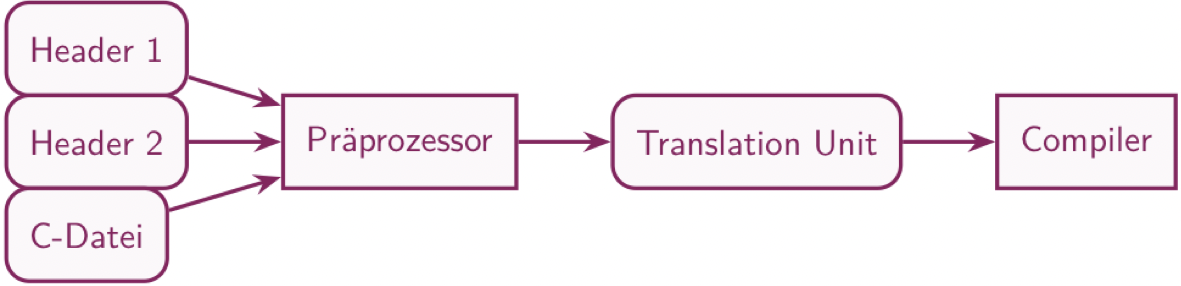
\includegraphics[width=0.75\linewidth]{translationunit}\\
%Globale Variablen
\textbf{Globale Variablen}
Haben immer einen Typ und einen Bezeichner und werden vor dem Main und ausserhalb von Funktionen definiert. Umfasst einen Speicherbereich mit einem Label darauf. Mit einem Header kann sichergestellt werden, dass mehrere C-Dateien dieselbe Deklaration sehen. Wird eine Globale Variable nicht definiert erhält sie Wert 0.\\
\begin{minipage}[b]{0,3\linewidth}
\begin{verbatim}
int x = 12;
\end{verbatim}
\end{minipage}
\begin{minipage}[b]{0,3\linewidth}
\begin{verbatim}
global x
x: dd 15
\end{verbatim}
\end{minipage}
\begin{minipage}[b]{0,3\linewidth}
Definition einer globalen Variable in C und Assembler.
\end{minipage}\\
\textbf{Lokale Variablen} Leben innerhalb einer Funktion und müssen bei jedem Funktionsaufruf neu angelegt werden.
\textbf{Objekte} sind ein zusammenhängender Speicherbereich.\\
\textbf{Variablen} Jede Variable ist ein Objekt, aber nicht jedes Objekt muss einer Variable entsprechen. Rückgabewerte von Funktionen werden in Objekten zurückgegeben. \\
\textbf{Typen} C kennt verschiedene Arten von Typen: Basistypen, Abgeleitete Typen, Enumerationen. Diese hängen von der verwendeten Maschine sowie Compiler ab.\\
\begin{minipage}[b]{0,5\linewidth}
\begin{verbatim}
sizeof(T) 
sizeof(char) = 1;
\end{verbatim}
\end{minipage}
\begin{minipage}[b]{0,5\linewidth}
Die Grösse von Typen wird in vielfachen von char angegeben. Auf Intel 64 1 Byte.
\end{minipage}
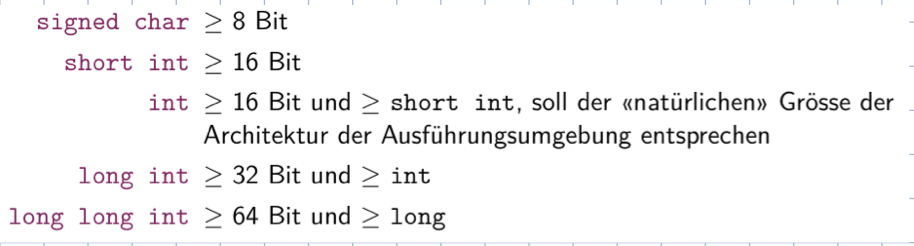
\includegraphics[width=\linewidth]{basistypen}
\textbf{Ausdrücke}
C übernimmt die Verwaltung der Register. Stattdessen schreiben wir Formel-ähnliche Ausdrücke. Jeder Ausdruck hat einen Typen, den der Compiler aus den Operanden ableitet (Konstanten, Literale, Bezeichner).\\
\textbf{Pointer}
Auf Maschienencodeebene gibt es keine Variablen, sondern nur Adressen. Die Adresse eines Objektes, dessen Typ nicht bekannt ist, ist vom Typ (void *). Die Addition eines integers zu einem Pointer berücksichtigt sizeof(T)\\ 
Die Adresse eines Objektes vom Typ T ist vom Typ *.
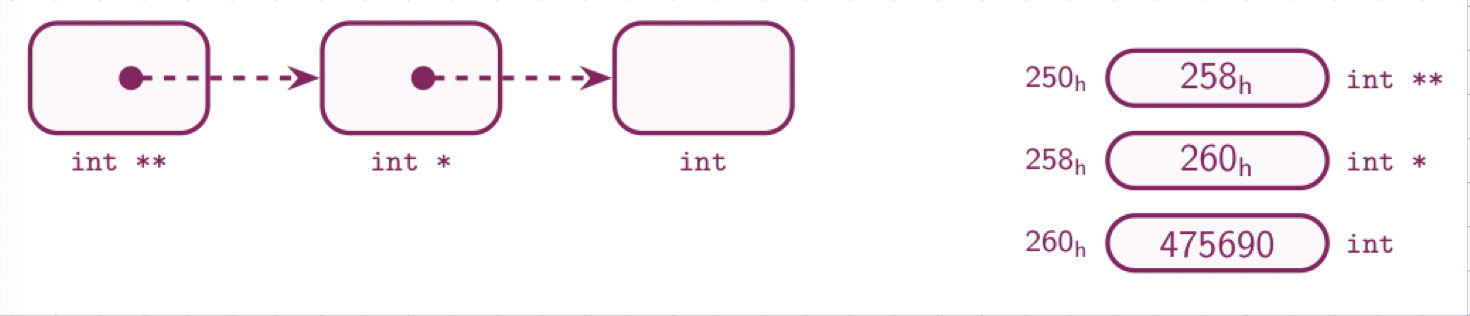
\includegraphics[width=\linewidth]{pointer}
\begin{minipage}[b]{0,3\linewidth}
\begin{verbatim}
int x = 5;
int *px = &x;
px = &x;
int y = *px;
\end{verbatim}
\end{minipage}
\begin{minipage}[b]{0,65\linewidth}
\& erzeugt die Adresse eines Ausdruckes.\\
Pointer syntax [Datentyp *Bezeichner]\\
Adresse an Pointer zuweisen\\
Asterisk * dereferenziert einen Pointer.
\end{minipage}
\textbf{Interpretation von Addressen} In C bedeutet: T * a\\
a = enthält die erste Andre eines Speicherbereichs m\\m = umfasst sizeof(T) Maschienenbytes. (a bis a + sizeof(T)-1) \\
\textbf{Index-Operatoren} a[b] ist definiert als *(a + b) \\
Ein Operand miss eine typisierte Andre sein (a)
Der andere Operand (b) muss ein Integer sein
%Asterisk
\\ Das \textit{Asterisk *} hat mehrere Bedeutungen. Es bezeichnet den Typ Pointer. Als Operator dereferenziert er eine Adresse. Im Arithmetischen beutetet er multiplizieren.\\
%Arrays
\textbf{Arrays} \\
\begin{minipage}[b]{0,5\linewidth}
\begin{verbatim}
T var[n]
int32_t a[10]
a[1] = 0x42;
\end{verbatim}
\end{minipage}
\begin{minipage}[b]{0,5\linewidth}
Definition\\\\
Labels eines Arrays als Pointer
\end{minipage}
Die Grösse eines Arrays gibt die Anzahl Maschienebytes zurück. Die Anzahl Elemente erhält man (Arraygrösse / Elementgrösse)\\
\textbf{size\_t} Unsigned Datentyp, der gross genus ist, um Grösse beliebiger Objekte zu halten. (Auch Iteration über Arrays)\\
\textbf{Null-terminierte Strings} char-Array, in welchem das letze Element \textbackslash0  (ASCII 0) ist.\\
\textbf{String-Literale} Entsprechen einer Sequenz von char und enden mit einer impliziten \textbackslash0. Werden an einem speziellen Ort gespeichert.
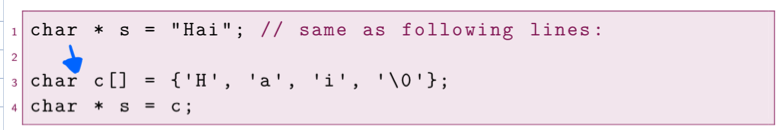
\includegraphics[width=\linewidth]{stringliterale}\\
\textbf{Const (Konstanten)} Definiert einen Wert, der nach der Initialisierung nicht mehr geändert werden kann. Der Wert kann sich durch äussere Einflüsse ändern.\\
\textbf{Strict (Strukturierte Variablen)} Strukturierte globale Variablen mit verschiedenen Datentypen. \\
\textit{vollständiger Struct:} Compiler hat genug Informationen um die Grösse eines Objektes zu bestimmen. \textit{unvollständige Typen} werden durch Forward-Deklaration eingeführt.\\
\textbf{Grundbegriffe der Logik}\\
\textit{Logische Funktion} Funktion von n Bits auf 1 Bit. \textit{Parameter} Variable zur Übergabe von Werten an eine Funktion. \textit{Argument} Wert eines Parameters bei konkreter Verwendung der Funktion.\\
\textit{Arität von Funktionen:} Es gibt vier unäre Funktionen (False(x), True(x), id(x), not(x).\\
Es gibt nulläre (null Parameter), Unäre, Binäre, Tender und n-Äre  Funktionen.
XOR, NAND - wichtige binäre Funktionen
Grössere Zahlen als Argumente - Funktionen müssen nicht von allen Bits abhängig sein.
Bitwise AND, OR, NOR\\
\textbf{Bitwise und Logische Operatoren in C}\\
\begin{minipage}[b]{0,4\linewidth}
\begin{verbatim}
not: z = ~q
and: z = q & p
or: z = q | p
xor: z = q ^ p
\end{verbatim}
\end{minipage}
\begin{minipage}[b]{0,4\linewidth}
\begin{verbatim}
Logische Operatoren:
z = !q
z = q && a
z = q || a
\end{verbatim}
\end{minipage}\\
\textbf{Funktionen}
% Shifts in C
\textbf{Shifts in C}\\
\begin{minipage}[b]{0,2\linewidth}
\begin{verbatim}
z = q << p
z = q >> p
\end{verbatim}
\end{minipage}
\begin{minipage}[b]{0,8\linewidth}
Beim Rechts-Shift wählt der Compiler die Instruktion abhängig vom Typ. (Unsigned:shr/Signed:sar) Einen Signed Links-Shift gibt es nicht.
\end{minipage}\\
%Funktionen
\textbf{Funktionen}
Aller ausführbarer Code in C muss in Funktionen stehen. \textit{Funktionsdeklaration:} Typ des Rückgabewertes, Bezeichner, Parameterliste in Klammern. Funktionen mit dem Typ void sind leer, aber Funktion mit () kann die Parameterliste irgendwas sein. Jede Funktion hat eine Adresse somit kann diese als Variable gespeichert werden.\\
\textbf{Funktion printf} \\
\begin{minipage}[b]{0,4\linewidth}
Dient der Ausgabe auf stdout und in stdio.h definiert.
\end{minipage}
\begin{minipage}[b]{0,6\linewidth}
\begin{verbatim}
int i = 20;
printf("Integer = %d \n", i);
\end{verbatim}
\end{minipage}
Die Format-Zeichen für die Funktion printf.\\
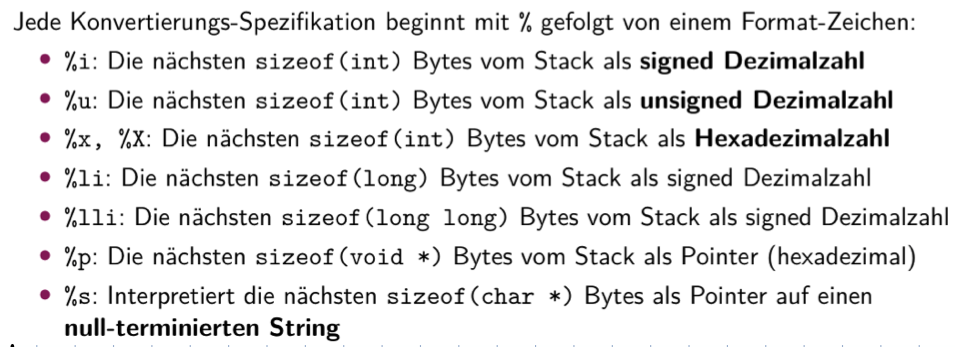
\includegraphics[width=\linewidth]{printf}\\
\textbf{Datentypen} Existieren nicht auf Maschinen-Code-Ebene. \textit{Maschinen-Byte:} kleinste Menge an Bits mit eigener Adresse (Intel64: 8). \textit{Maschinen-Wort:} grösste Menge an Bits, die ein Prozessor in einem Zyklus bearbeiten kann.\\
\textbf{Typen-Alias} Mit typedef kann ein bestehender Typ einen weiteren Namen (Alias) erhalten. Der Compiler behandelt alle Aliase gleich.Es gibt vordefinierte Aliase.\\
%Stack
\subsection{Stack}
\vspace{-0.75em}
Umfasst einen Stackpointer, Operationen: push, pop. \textit{Intel Stack}: Hat 8 Byte grosse Elemente, Oberste E. liegt an niedrigster Adresse, Der Stack wächst in Richtung der niedrigsten Adresse. Der Stackpointer (RSP) zeigt immer auf das zuletzt abgelegte Objekt. \\
\textbf{Push}\\
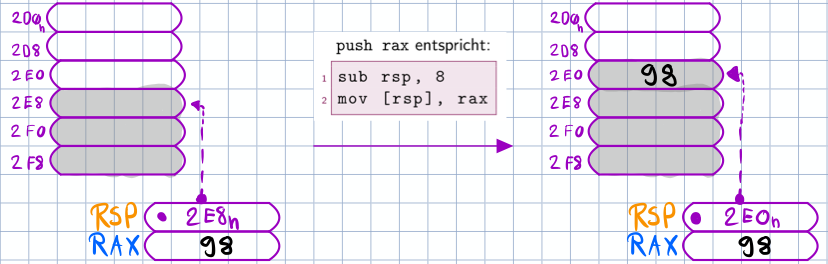
\includegraphics[width=\linewidth]{stackpush}
\textbf{Pop}\\
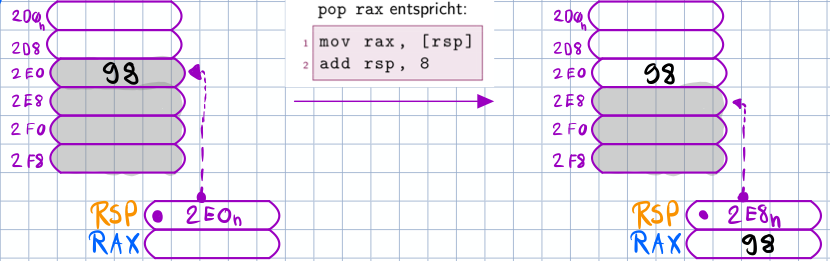
\includegraphics[width=\linewidth]{stackpop}\\
%Stack Assembler
\textbf{Call und RET}
Call a: Nachfolgende Adresse r auf den stack und Sprung an a. Ret: Adresse r von Stack und Sprung nach r\\
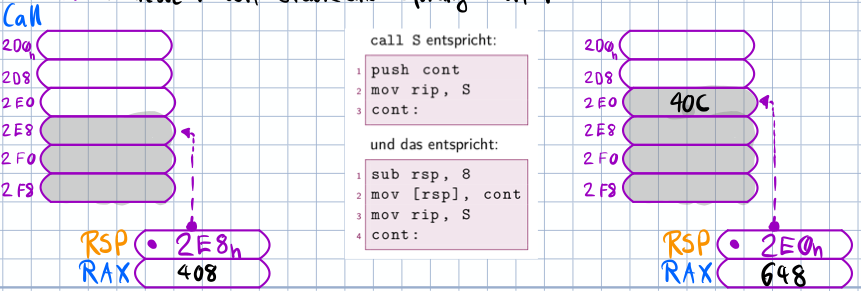
\includegraphics[width=\linewidth]{stackcallret}
%Frame Pointer
\textbf{Frame Pointer}\\
Die Adressen des Stacks sind relativ zum Frame Pointer. Dafür wird für den Stack ein Prolog und Epilog benötigt.\\
\begin{minipage}[b]{0,5\linewidth}
\begin{verbatim}
push rbp
mov rbp, rsp
\end{verbatim}
\end{minipage}
\begin{minipage}[b]{0,5\linewidth}
\begin{verbatim}
mov rsp, rbp
pop rbp
\end{verbatim}
\end{minipage}\\
\textbf{Calling Convention}
Vereinbarung zwischen Caller und Calle, welche Register die Funktion verändern darf und in welchen Registern die Argumente der Funktion übergeben werden.

% Mathematische Grundlagen
\subsection{Mathematische Grundlagen}
\vspace{-0.75em}
\begin{minipage}[b]{0,5\linewidth}
\textbf{Addiditon}
Funktioniert wie bei den Dezimalzahlen.\\\\
\end{minipage}
\begin{minipage}[b]{0,5\linewidth}
\textbf{Subtraktion}
Ist der Miuend kleiner als der Subtrahend, erhöht man den Minuenden um 2\^ n auf eine (n+1)-stellige Zahl.
\end{minipage}\\
\textbf{Vorzeichenbehaftete Ganzzahlen}\\
\textit{Unsigned Integer:} Wertebereich: 0 bis $2^{n}-1$\\
\textit{Signed Integer:} Wertebereich: $-(2^{n-1})$ bis $-(2^{n-1})-1$\\
\textbf{Einer- und Zweierkomplement}\\
Sind in der läge auch negative Zahlenwerte darzustellen. Im Einerkomplement wird das MSB als Vorzeichen interpretiert. Problem - zwei mögliche Nullen. Das Zweierkomplement behebt dies.\\
\textit{Inversionsverfahren 1:} b - 1, invertieren\\
\textit{Inversionsverfahren 2:} b invertieren, b + 1\\
\textbf{Arithmetische Operationen in Assembler und C}\\
\begin{minipage}[b]{0,4\linewidth}
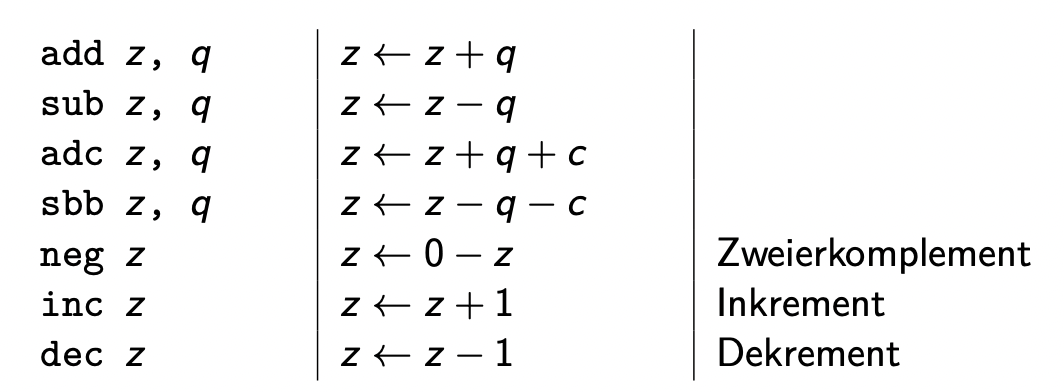
\includegraphics[width=\linewidth]{armassembler}
\end{minipage}
\begin{minipage}[b]{0,6\linewidth}
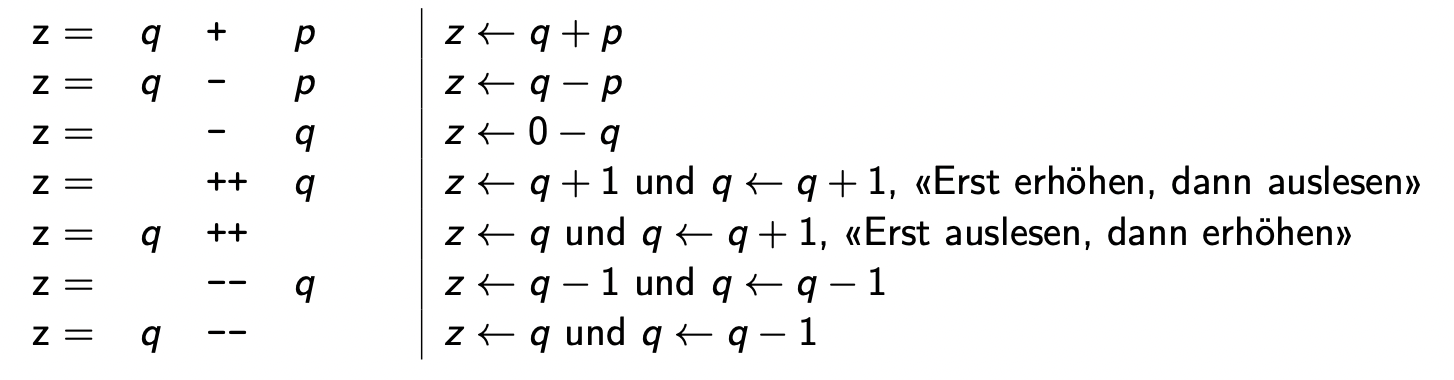
\includegraphics[width=\linewidth]{armc}
\end{minipage}\\
\textbf{Links- und Rechts-Shift}\\
\textit{Links-Shift um n Bits:} $b * 2^{n}$,
\textit{Rechts-Shift um n Bits:} $b / 2^{n}$\\
\textbf{Sign-Extension}
Wenn eine n-Bit Zahl auf eine n+m-Speicherstelle kopiert wird, werden die oberen m Bits auf 0 gesetzt. Dies ändert  die Bedeutung der Zahl (wenn sie im Zweierkomplement geschrieben ist).
Die Sign-Extension füllt die oberen m Bits mit 1-en auf.\\
\textbf{Shifts und Rotate in Assembler}
Rotates füllen statt mit 0 oder 1 mit den ursprünglichen Bits auf.\\
%  Assembler multiplikation und division
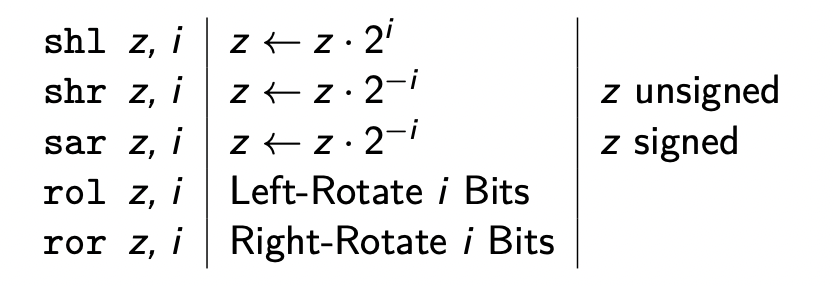
\includegraphics[width=0.5\linewidth]{shrt}\\
\textbf{Signed Multiplikation in Assembler}\\
\begin{minipage}[b]{0,2\linewidth}
\begin{verbatim}
imul r, z 
mul r, z 
\end{verbatim}
\end{minipage}
\begin{minipage}[b]{0,8\linewidth}
\textit{imul} ist das signed Äquivalent zu \textit{mul} auf Assembler.
\end{minipage}\\
\textbf{Signed Divison in Assembler}\\
\begin{minipage}[b]{0,2\linewidth}
\begin{verbatim}
idiv r, z 
div r, z 
\end{verbatim}
\end{minipage}
\begin{minipage}[b]{0,8\linewidth}
\textit{idiv} ist das signed Äquivalent zu \textit{div} auf Assembler.
\end{minipage}

%Speicher und Cache
\subsection{Hauptspeicher und Cache}
\vspace{-0.75em}
\textbf{Physikalische Grenzen der Computertechnik} Elektrische Energie 2/3 der Lichtgeschwindigkeit. Somit kann eine 3GHz CPU pro Takt nur 10cm weit kommunizieren. CMOS-Logik verbraucht Energie, wenn Transistoren schalten.\\
\textbf{Speicherhierarchien} Ein Computer Verwendet verschiedene Arten von Speicher. Höherwertiger Speicher: (Ram, Cache): niedrige Distanz CPU, Hohe Geschwindigkeiten, Geringe Fehleranfälligkeit, Geringe Sicherheitsanforderungen, Niederwertiger Speicher: (Tape, HDD): Preis, Kapazität, Transfereinheiten.\\
\textbf{Lokalitätsdiagramm} Speicherzugriff im zeitlichen Verlauf. Arbeitsbereich W(t, delta t). \textit{Räumliche Lokalität:} Arbeitsbereich enthält nahe beieinander liegende Speicherstellen. \textit{Zeitliche Lokalität:} Auf Speicher, auf den kürzlich zugegriffen wurde, wird bald wieder zugegriffen.\\
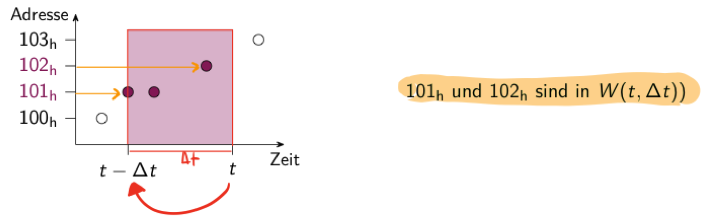
\includegraphics[width=\linewidth]{arbeitsbereich}\\
\textbf{Cache} ist ein Zwischenspeicher, der kleiner und schneller ist. \textit{Nutzen:} Ergibt sich aus dem Lokalitätsprinzip. \\
\textbf{Durchschnittliche Zugriffszeit} \\
E(T) = p$_{c}$ * T$_{c}$ + (1 - p$_{c}$) * T$_{m}$ \\
T$_{c}$ = Zugriffszeit auf den Cache\\
T$_{m}$ = Zugriffszeit auf den Hauptspeicher\\
p$_{c}$ = Wahrscheinlichkeit eines Cache-Hits (oft $>$ 0.9)\\\\
\textbf{Fully-Associate-Caches}\\
\textit{Chachezeilen:} besteht aus 64 Byte. Somit umfasst jede Cachezeile die Adressen c$_{k}$+0 bis c$_{k}$+63.\\
Die Adresse Besteht aus Tag und Offset. Das Tag der Zeile sind die oberen (n-6) bits t$_{k}$ = c$_{k}$ / 2$^{6}$, Offset = untere 6 Bits.\\
Nutzen den Lokalitätseffekt best-möglich aus, sind aber teuer zu implementieren.\\
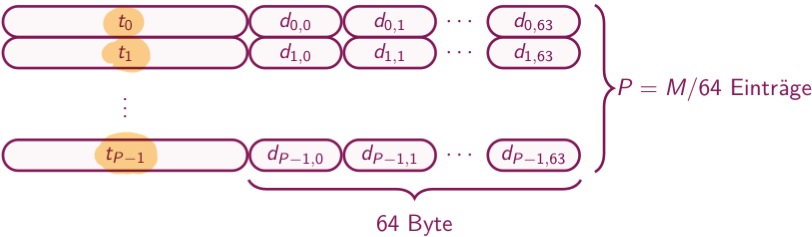
\includegraphics[width=\linewidth]{fullyassociative}\\
\textbf{Direct-Mapped Caches}\\
Der DMC ist sehr einfach zu implementierender Cache mit einem schnellen Lookup. Hat aber viele Kollisionen.\\
Die Adresse besteht aus Tag, Index, Offset.\\
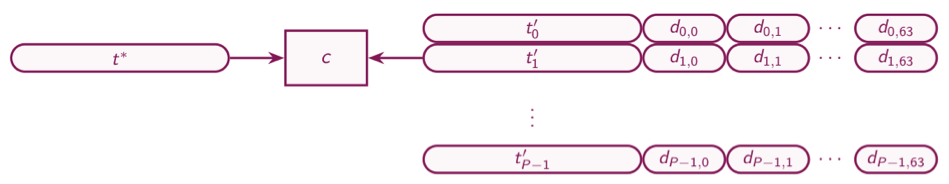
\includegraphics[width=\linewidth]{dmc}\\
% K-way set associative
\textbf{k-way Set-Associative Cache}\\
Eine parallele Verwendung von k Direct-Mapped Caches mit jeweils P / k Einträgen. Jede Chachezeile kann ich k verschiedenen Cacheeinträgen gespeichert werden. (Set) Der SAC ist ein Kompromiss zwischen FAC und DMC: weniger komplex als FAC, weniger Kollisionen als DMC, genauso schnell wie FAC und DMC. Eine stelle teilt sich ($HS * ways$ / Cachegrösse mit WAY-stellen den Platz).
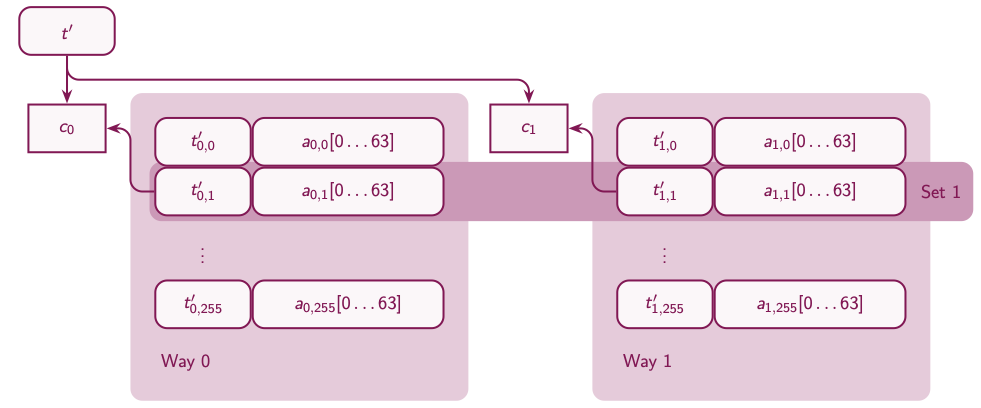
\includegraphics[width=\linewidth]{2-wayset}

\subsection{Dynamischer Speicher}
\vspace{-0.75em}
Der Heap ist ein Speicherbereich für vollständig dynamischen Speicher. Dieser wird vom OS verwaltet.\\ 
\textbf{Implizite Speicherfreigabe}\\
Virtuelle Laufzeitumgebungen (Java, .NET) schränken Pointer stark ein. Dafür gibt es keine Speicherlecks. Keine Kontrolle über Zeitpunkt Speicherfreigabe,
Zeitverhalten inderterministisch,
Zeit- und Speicheroverhead zur Laufzeit.\\
\textbf{Explizite Speicherfreigabe}\\
Programmiere bestimmt Zeitpunkte für Speicherfreigabe und Reservationen explizit. (In C malloc und free). Beachten das die Dualität beibehalten wird.
\textbf{Interne Fragmentierung} Wenn eine Heap-Implementierung einen grösseren Speicherblock reserviert als benötigt. \textit{Mögliche Lösung:} Programm übernimmt selbst feingranulare Verwaltung (Java, .NET, DBMS) \textbf{Externe Fragmentierung} Programm reserviert immer wieder Speicher und gibt ihn unregelmässig frei. Programmierer können das Problem umgehen. (Object Pools, Komposition statt Aggregation).\\
\textbf{Suchalgorithmen}\\
\textit{First Fit:} Wählt erste passende Lücke am Anfang. \textit{Next Fit:} Wählt erste passende Lücke nach zuletzt reservierten Bereich. \textit{Best Fit:} Durchsucht alle Lücken und wählt beste aus. \textit{Worst Fit:} Durchsucht alle Lücken und wählt grösste aus. \textit{Quick Fit:} Wählt erstes passendes Element aus der Liste.\\
\textbf{Buddy-System} Variante des Verfahrens Grössenklassen mit Zweierpotenzen von 2$^{m}$ bis 2$^{n}$. (2$^{m}$ kleinste Speicherbereichsgrösse, 2$^{n}$ gesamter Speicher) Wird ein 2$^{k}$-Bereich in zwei 2$^{k-1}$-Buddies geteilt, müssen deren Startadressen die untersten k-1 Bits = 0.\\
\textbf{Object Pools} Ein Speicherbereich fester Grösse (Page) wird in kleinere Bereiche mit gleicher Grösse unterteil (Objekte).

\subsection{Virtueller Speicher HW}
\vspace{-0.75em}
\textbf{Virtuelle Adressen} Das OS gibt dem Prozess keine reale Adressen, sondern virtuelle. Die MMU übersetzt virtuelle in reale Adressen. (Physische = reale Adresse, logische = virtuelle = lineare Adresse) \\
\textit{Gültiger Zugriff:} Prozess will auf gültige Adresse zugreifen, MMU findet mapping in Mappingtabelle, MMU legt reale Adresse auf den Speicherbus, Prozessor lies/schreibt Daten von/auf Speicherbus. \textit{Ungültiger Zugriff:} Prozessor will auf ungültige Adresse zugreifen, MMU stellt fehlendes Mapping fest, MMU signalisiert Fault-Interrupt, CPU ruft OS-Interrupt-Handler auf, OS Memory Manager übernimmt.\\
\textit{Effekte:} Mehr Speicher pro Prozess (Prozess hat mehr Speicher als Hauptspeicher vorhanden), Mehr Speicher als reale Adressbits ermöglichen.\\
\textbf{Monoprogrammierung:} Der Prozess kennt keine anderen Prozesse\\
\textbf{Seitenbasierter Virtueller Speicher}
Verwaltungseinheit: Seite bzw. Page, typischerweise 4KB (entspricht 12 Bit offsets). Der Hauptspeicher besteht aus Page Frames. Die Page repräsentiert die Daten, Page ist kein Speicher, sondern benötigt einen Page Frame. Page Number = Startadresse der Page ohne Offsetbits. Das OS entscheidet, welche Pages wann wo liegen müssen. MMU kennt nur den Hauptspeicher und kann nur das Fehlen einer Page bemerken.\\
\subsection{Virtueller Speicher SW}
\vspace{-0.75em}
\textbf{Page-Table} Jede virtuelle Adresse wird via Page-Table in reale Adresse übersetzt. (Single-Level, Mutei-Level, Inverted, Hashtable) Jeder Eintrag id der Page-Table enthält zusätzlich zwei Statusbits. \textit{Translation Lookaside Buffer:} Cache für häufig benötigte Mappings (keine Daten).\\
\textbf{Paging}\\
Auf Intel x86 hat jeder Page-Table Eintrag 32 Bits. Das Unterste Bit ist das P-Bit (Present). Wenn dieses auf 1 steht, ist die Page im Hauptspeicher.  Zusätzlich gibt es das A-Bit und D-Bit.\\
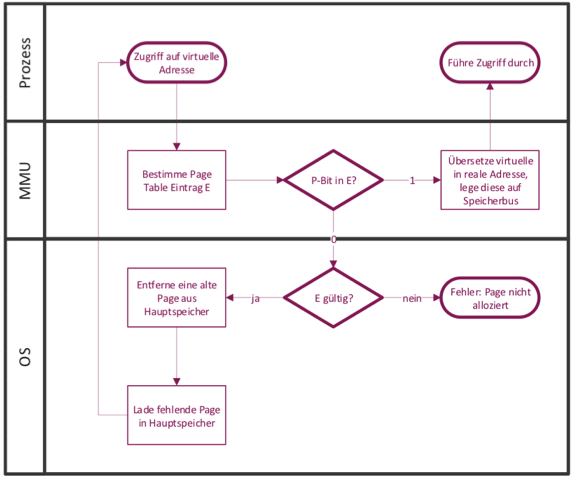
\includegraphics[width=0.6\linewidth]{paging}
\begin{minipage}[b]{0,4\linewidth}
\textbf{Ablauf im Interrupt}\\
OS prüft, ob Lokalisierungsinformationen gültig sind. Wenn HS voll, OS entscheide, welche Page entfernt werden soll. OS initiiert Page-Transfer von sekundärem Speicher. In der Zwischenzeit laufen die Prozesse weiter.\\
\textit{Page geladen} OS setzt Prozess mit Instruktion fort.
test
\end{minipage}\\
\textbf{Dreschen (Threshing)}\\
Bschreibt das Problem von zu häufigem Pagen. (HS zu klein, zu viele Prozesse)\\
\textbf{Teilstrategien} Ladestrategien (fetching policies), Entladestrategien (cleaning policies), Verdrängungsstrategien (page replacement policies)
\textbf{Ladestrategien} \textit{Demand Paging:} Laden auf Anfrage (minimaler Aufwand, lange Wartezeiten). \textit{Prepaging:} Pages werden frühzeitig geladen durch statistische Systemanalyse (In der Praxis nicht anzutreffen). \textit{Demand Paging mit Prepaging:} Laden auf Anfrage und benachbarte Pages werden mitgeladen. Pages werden in Clustern geladen (4-8). (Weniger Page-Faults, Bocktransfer, möglicherweise zu viele Pages)\\
\textbf{Entladestrategien}\\
\textit{Demand Cleaning:} Entladen auf Nachfrage. Page wird zurückgeschrieben, wenn Frame wieder verwendet werden soll. (Minimaler Aufwand, Erhöhte Wartezeit) \textit{Precleaning:} Modifizierte Pages werden frühzeitig in den sekundären Speicher geschrieben. (Reduzierte Wartezeit, Mehraufwand) \\
\textbf{Veränderungsstrategien}\\
Zahlreiche Varianten: FIFO, Second Chance, Clock. Massiver Einfluss auf die Systemperformance. MMU setzt die Statusbits und das OS löscht sie.\\
\textit{Optimum:} Ersetzt die Pages, die am spätesten in der Zukunft gebraucht wird.
\textit{FIFO:} Ersetzt jeweils die älteste Seite. Benötigt keine Statusbits. Problem der Bélàdys Anomalie: Grösserer HS kann zu mehr Page Faults führen.\\
\textit{Second Chance:} Erweiterung von FIFO. Prüft A-Bit der ältesten Page. Wenn A = 0 - Entladen der Page. Wenn A = 1, OS löscht A-Bit und schiebt Page ans ende der Linked List.\\
\textit{Clock:} Linked-List wird zum Kreis (=Clock) und ein Pointer wird verwendet.\\
\textit{LRU - Last Recently Used:} Ersetzt die am längsten unbenutzte Page. Bei jedem Zugriff notiert MMU den Zeitpunkt.  (Grosse Aufwand in Hardware)\\
\textit{NFU - Not Frequently Used:} Benötigt einen zusätzlichen Counter in der Page-Table. Wenn es einen oder mehere Zugriff*e gab, Counter erhöht. Ersetzt die Page mit dem niedrigstem Counter. Problem: alte pages können lange bleiben.\\
\textit{NFU mit Aging:} Counter gewichtet nach Zeit. Pro Page ein n-Bit counter.\\
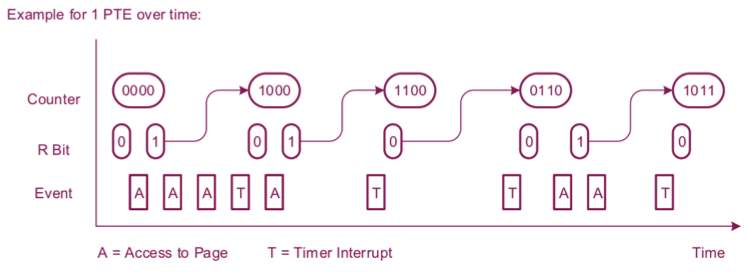
\includegraphics[width=\linewidth]{nfuaging}
\textit{Working Set:} Behalte Pages vom Working Set (mit Intervall T). Pro Page-Table-Eintrag ein Zeitstempel T. Statt Timer-Interrupt: Scanne alle Pages mit Fault-Interrupt. Wenn A = 1, setze t = now, und A = 0. Wenn A = 0, wenn now -t $<$T Page im WS und bleibt oder -t $>=$ T Page nicht im WS und wird entfernt.\\

\end{multicols*}
\end{document}  